\documentclass{article}
\usepackage[utf8]{inputenc} % Para soportar caracteres en español
\usepackage{amsmath, amssymb} % Para \mathbb{R}
\usepackage{tikz}
\usetikzlibrary{shapes, arrows, positioning}
\usepackage{caption}

\newenvironment{definition}[1][Definición]{\begin{trivlist}
\item[\hskip \labelsep {\bfseries #1}]}{\end{trivlist}}

\newenvironment{remark}[1][Observación]{\begin{trivlist}
\item[\hskip \labelsep {\bfseries #1}]}{\end{trivlist}}


\begin{document}

\chapter{Análisis, Diseño e Implementación de Sistemas de Información Analíticos (OLAP)}

Habiendo establecido el formalismo para los sistemas que capturan el estado transaccional de un dominio, ahora dirigimos nuestra atención a los sistemas diseñados para analizar la evolución temporal de dicho estado. Los sistemas de Procesamiento Analítico en Línea (OLAP) no se ocupan de registrar operaciones atómicas, sino de la agregación, el descubrimiento de patrones y el modelado de datos históricos a gran escala. Este es el dominio de la Inteligencia de Negocios (BI).

\section{Problemas y Desafíos en la Inteligencia de Negocios}
La transición de la recolección de datos a la extracción de conocimiento accionable no es trivial. Requiere una arquitectura fundamentalmente diferente y un reenfoque del modelado, pasando de la normalización para la eficiencia de escritura a la desnormalización para la eficiencia de lectura agregada.

\subsection{Conceptos Básicos}
\begin{definition}[Inteligencia de Negocios (BI)]
La Inteligencia de Negocios es un paradigma que abarca un conjunto de teorías, metodologías, arquitecturas y tecnologías que transforman datos crudos en información y conocimiento significativo y útil para propósitos de análisis y toma de decisiones estratégicas en una organización. Mientras que los sistemas OLTP responden a la pregunta "¿Cuál es el estado actual del sistema?", los sistemas de BI responden a "¿Cuáles son las tendencias y patrones que emergen de la historia de los estados del sistema?".
\end{definition}

\begin{definition}[Procesamiento Analítico en Línea (OLAP)]
OLAP es la tecnología subyacente que permite el análisis rápido, interactivo y multidimensional de grandes volúmenes de datos. Un "cubo" OLAP es la estructura de datos conceptual que permite este análisis, representando los datos a través de \textbf{dimensiones} (ejes de análisis, p. ej., tiempo, geografía, producto) y \textbf{medidas} (valores numéricos a ser agregados, p. ej., ventas, ingresos).
\end{definition}

El desafío fundamental es que los datos generados por los sistemas OLTP no están estructurados para el análisis. Están altamente normalizados para minimizar la redundancia y optimizar las escrituras, lo que resulta en esquemas complejos de docenas o cientos de tablas. Una consulta analítica simple ("¿Cuáles fueron las ventas totales por región en el último trimestre?") requeriría un número prohibitivo de operaciones de join sobre estos esquemas, resultando en un rendimiento inaceptable.

\subsection{Arquitectura Canónica de un Sistema de BI}
Para resolver este problema, se postula una arquitectura desacoplada, donde los datos operacionales son periódicamente extraídos, transformados y cargados en un repositorio central optimizado para el análisis.

\begin{center}
\resizebox{0.9\textwidth}{!}{%
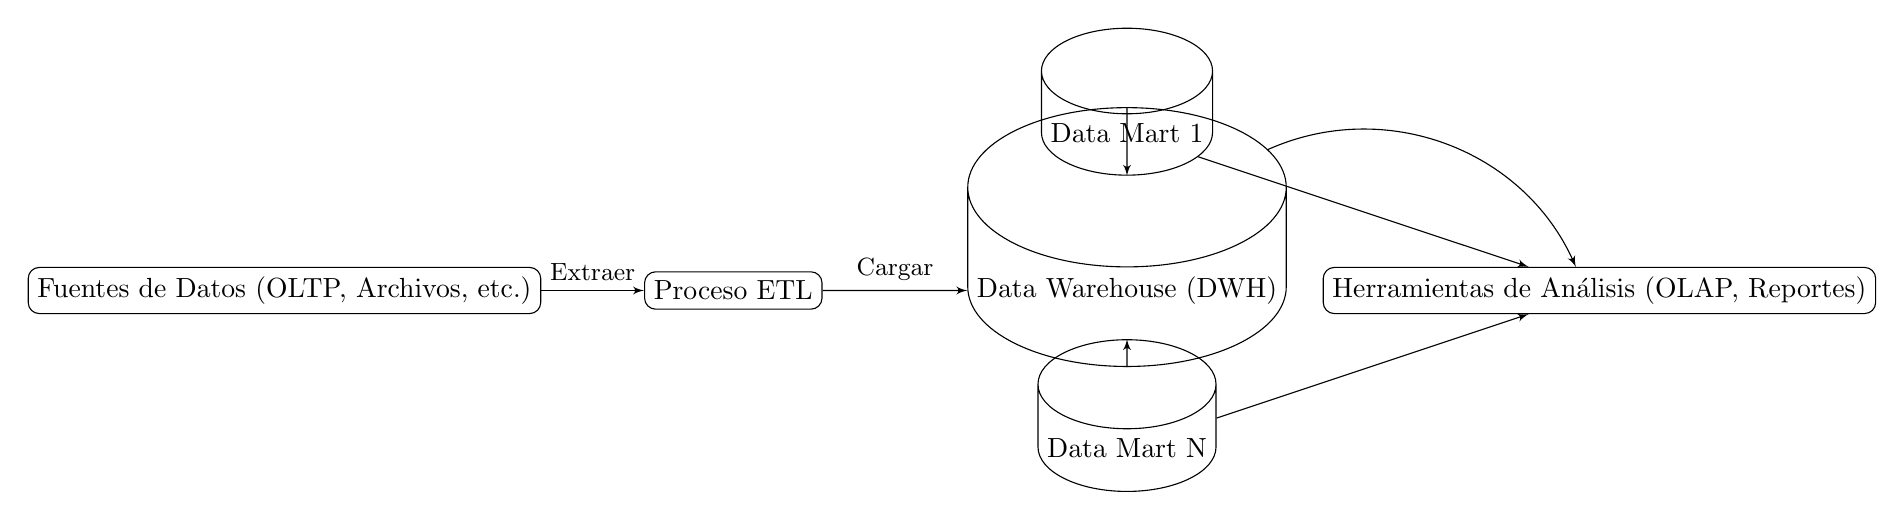
\begin{tikzpicture}[node distance=2.5cm, auto, >=latex']
    \node[draw, rectangle, rounded corners] (sources) {Fuentes de Datos (OLTP, Archivos, etc.)};
    \node[draw, rectangle, rounded corners, right of=sources, xshift=3.2cm] (etl) {Proceso ETL};
    \node[draw, cylinder, shape border rotate=90, aspect=0.5, right of=etl, xshift=2.5cm] (dwh) {Data Warehouse (DWH)};
    \node[draw, cylinder, shape border rotate=90, aspect=0.5, above of=dwh, yshift=-0.5cm] (dm1) {Data Mart 1};
    \node[draw, cylinder, shape border rotate=90, aspect=0.5, below of=dwh, yshift=0.5cm] (dm2) {Data Mart N};
    \node[draw, rectangle, rounded corners, right of=dwh, xshift=3.5cm] (analysis) {Herramientas de Análisis (OLAP, Reportes)};
    
    \path[->] (sources) edge node[midway, above, font=\small] {Extraer} (etl);
    \path[->] (etl) edge node[midway, above, font=\small] {Cargar} (dwh);
    \path[->] (dwh) edge (dm1);
    \path[->] (dwh) edge (dm2);
    \path[->] (dm1) edge (analysis);
    \path[->] (dm2) edge (analysis);
    \path[->] (dwh) edge [bend left=45] (analysis);
\end{tikzpicture}%
}
\end{center}

\begin{description}
    \item[Fuentes de Datos:] Los sistemas OLTP, hojas de cálculo, logs de servidores, etc., que generan datos operacionales.
    \item[Proceso ETL (Extraer, Transformar, Cargar):] El núcleo del sistema.
    \begin{itemize}
        \item \textbf{Extraer:} Obtención de los datos desde las fuentes.
        \item \textbf{Transformar:} La fase más compleja. Incluye la limpieza de datos (manejo de nulos, corrección de errores), integración (unificación de datos de múltiples fuentes) y desnormalización para crear un \textbf{modelo dimensional}.
        \item \textbf{Cargar:} Inserción de los datos transformados en el Data Warehouse.
    \end{itemize}
    \item[Data Warehouse (DWH):] Un repositorio de datos central, integrado, histórico y no volátil. Es la "única fuente de la verdad" para toda la organización.
    \item[Data Marts:] Subconjuntos del DWH, orientados a un área de negocio específica (p. ej., Ventas, Finanzas), para simplificar el acceso y mejorar el rendimiento.
\end{description}

\subsection{¿Qué es un Modelo de Negocio?}
Antes de que cualquier dato pueda ser analizado, es imperativo entender formalmente el dominio que lo genera. Un modelo de negocio es un cianotipo conceptual que describe la lógica de cómo una organización crea, entrega y captura valor. Aunque no es una fórmula matemática rígida, puede ser deconstruido en un conjunto de componentes centrales e interconectados. El marco formal más aceptado para esto es el Business Model Canvas, que define un modelo de negocio a través de nueve bloques de construcción:

\begin{description}
    \item[Segmentos de Clientes] Los distintos grupos de personas u organizaciones que una empresa pretende alcanzar y servir.
    \item[Propuestas de Valor] El conjunto de productos y servicios que crean valor para un Segmento de Clientes específico. Es la razón por la cual los clientes eligen una compañía sobre otra.
    \item[Canales] Describe cómo una compañía se comunica y llega a sus Segmentos de Clientes para entregar una Propuesta de Valor.
    \item[Relaciones con Clientes] Los tipos de relaciones que una compañía establece con Segmentos de Clientes específicos (p. ej., transaccional, a largo plazo, automatizada).
    \item[Fuentes de Ingresos] El efectivo que una compañía genera de cada Segmento de Clientes. Representa el valor capturado.
    \item[Recursos Clave] Los activos más importantes requeridos para que el modelo de negocio funcione (p. ej., físicos, intelectuales, humanos, financieros).
    \item[Actividades Clave] Las acciones más importantes que una compañía debe realizar para operar exitosamente (p. ej., producción, resolución de problemas, gestión de plataformas).
    \item[Asociaciones Clave] La red de proveedores y socios que hacen que el modelo de negocio funcione.
    \item[Estructura de Costos] Todos los costos incurridos para operar un modelo de negocio.
\end{description}

El propósito de un sistema de inteligencia de negocios es cuantificar el rendimiento y la interacción de estos nueve bloques. Por ejemplo, un sistema de BI puede medir la rentabilidad de diferentes \textbf{Segmentos de Clientes}, la efectividad de varios \textbf{Canales}, o la eficiencia en costos de las \textbf{Actividades Clave}. El modelo de datos del sistema de BI debe ser diseñado para capturar las métricas que iluminan estos componentes fundamentales.

\subsection{Preguntas para Construir un Modelo de Negocio y BPMN}
El análisis de un modelo de negocio gira en torno a una serie de preguntas fundamentales: ¿Quiénes son nuestros clientes? ¿Qué valor les entregamos? ¿A través de qué canales? ¿Qué actividades clave requieren nuestros procesos?
Para modelar formalmente los procesos de negocio ($\mathcal{P}$), se utiliza un estándar gráfico llamado \textbf{Modelo y Notación de Procesos de Negocio (BPMN)}. BPMN es un lenguaje visual que permite la especificación de flujos de trabajo de manera análoga a como un diagrama de flujo especifica un algoritmo.

Sus elementos principales son:
\begin{itemize}
    \item \textbf{Eventos:} Círculos que representan algo que "sucede" (p. ej., pedido iniciado, pago recibido).
    \item \textbf{Actividades:} Rectángulos con esquinas redondeadas que representan trabajo que se "hace" (p. ej., verificar inventario, enviar producto).
    \item \textbf{Compuertas (Gateways):} Rombos que controlan la divergencia y convergencia del flujo (p. ej., decisiones, flujos paralelos).
    \item \textbf{Flujos de Secuencia:} Flechas que conectan los elementos precedentes.
\end{itemize}
% \begin{figure}[h]
%     \centering
%     % 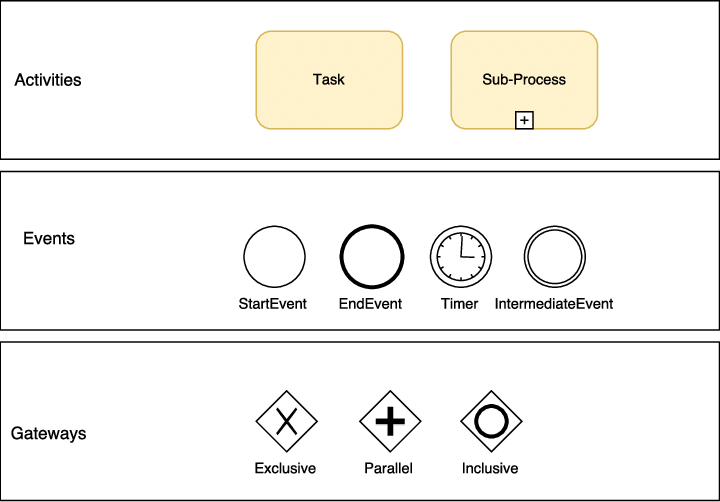
\includegraphics[width=0.5\linewidth]{Notation.png}
%     \caption{Notación extendida de BPMN}
%     \label{fig:placeholder}
% \end{figure}
Modelar en BPMN es el primer paso para identificar qué debe ser medido en una organización.

\subsection{Estableciendo Indicadores Clave de Desempeño (KPIs)}
Una vez que los procesos de negocio están formalmente definidos, es necesario cuantificar su rendimiento.
\begin{definition}[Indicador Clave de Desempeño (KPI)]
Un Indicador Clave de Desempeño (KPI) es una función $f: S \to \mathbb{R}$, donde $S$ es el espacio de estados de un proceso de negocio, que mapea el estado del proceso a un valor numérico cuantificable. Este valor se compara contra un objetivo predefinido para evaluar el rendimiento. Un KPI debe ser:
\begin{itemize}
    \item \textbf{Cuantificable:} Medible de forma numérica.
    \item \textbf{Accionable:} Su valor debe poder ser influenciado por las acciones de la organización.
    \item \textbf{Estratégico:} Debe estar directamente alineado con un objetivo de negocio.
\end{itemize}
\end{definition}
\textit{Ejemplos:} Tasa de Conversión de Ventas ( (Número de Ventas / Número de Prospectos) $\times$ 100), Costo de Adquisición de Cliente (Costo Total de Marketing / Número de Nuevos Clientes), Tiempo de Ciclo de Pedido.

La selección de los KPIs correctos es la culminación del análisis de requerimientos en un proyecto de inteligencia de negocios. Estos KPIs dictan qué medidas y dimensiones deben ser modeladas en el cubo OLAP, qué datos deben ser extraídos por el ETL y, en última instancia, qué conocimiento puede ser extraído del sistema.

\section{Análisis y Diseño del Data Warehouse}
La transición del dominio OLTP al dominio OLAP no es meramente un cambio de aplicación; es un cambio de paradigma fundamental en la filosofía del modelado de datos. Los esquemas altamente normalizados (3NF/BCNF), que son obras maestras de eficiencia para la integridad transaccional y la minimización de la redundancia, se convierten en un cuello de botella insuperable para las consultas agregadas complejas y a gran escala que definen la inteligencia de negocios. El objetivo ya no es la optimización de operaciones de escritura atómicas, sino la optimización de operaciones de lectura masivas y agregadas. Esto necesita un nuevo formalismo: el modelado multidimensional.

\subsection{El Paradigma del Modelado Multidimensional}
El modelado multidimensional es una metodología de diseño que estructura los datos no en torno a entidades atómicas y sus relaciones, sino en torno a los procesos continuos de un negocio y las mediciones numéricas discretas (eventos) que estos procesos generan. Proporciona un marco intuitivo y de alto rendimiento para consultas analíticas al abstraer los datos en una estructura análoga a un hipercubo geométrico.

\begin{definition}[Modelo Multidimensional]
Un modelo multidimensional es un modelo de datos que organiza los datos en un hipercubo lógico, o "cubo". Esta estructura n-dimensional consta de dos tipos de componentes fundamentales y ortogonales:
\begin{itemize}
    \item \textbf{Hechos (Facts):} Las mediciones numéricas que corresponden a un evento específico dentro de un proceso de negocio. Estos forman el cuerpo cuantitativo del cubo.
    \item \textbf{Dimensiones:} El contexto categórico que define los ejes de coordenadas del hipercubo. Proporcionan el contexto de "quién, qué, dónde, cuándo, por qué" para los hechos.
\end{itemize}
Una consulta analítica, por lo tanto, ya no es un recorrido complejo de un grafo de tablas normalizadas, sino más bien un "corte" (slice) o una agregación a través de un sub-volumen de este hipercubo.
\end{definition}

\subsection{Los Componentes Axiomáticos: Hechos y Dimensiones}
La separación limpia y ortogonal entre hechos (lo que se mide) y dimensiones (el contexto de la medición) es el axioma fundamental del modelado dimensional.

\subsubsection{Tablas de Hechos y sus Tipos}
Un hecho representa un evento específico y cuantificable. Estos eventos se almacenan en una \textbf{tabla de hechos} central. Cada fila en esta tabla corresponde a una medición discreta en un punto específico en el espacio n-dimensional definido por las dimensiones. Las tablas de hechos son el centro gravitacional del modelo.

\begin{description}
    \item[Granularidad:] El concepto más importante en el modelado dimensional. El \textbf{grano} de la tabla de hechos es una declaración formal de lo que representa una sola fila (p. ej., "un ítem de línea de producto individual en el recibo de venta de un cliente"). Toda decisión de diseño fluye de esta declaración.
    \item[Medidas:] Los atributos numéricos que cuantifican el evento. Se clasifican por su aditividad: \textbf{totalmente aditivas} (p. ej., `cantidad_vendida`), \textbf{semi-aditivas} (p. ej., niveles de inventario, que no son aditivos a través del tiempo), y \textbf{no aditivas} (p. ej., ratios, que deben ser calculados a partir de componentes aditivos).
\end{description}

Existen tres tipos canónicos de tablas de hechos, distinguidos por cómo registran las mediciones a lo largo del tiempo:
\begin{description}
    \item[Tablas de Hechos Transaccionales] Este es el tipo más común y fundamental. Cada fila corresponde a un único evento en un único punto en el tiempo, representando una medición instantánea. La tabla crece añadiendo continuamente nuevas filas a medida que ocurren los eventos. El grano es típicamente de bajo nivel, capturando el nivel más atómico de un proceso de negocio. El ejemplo de `Fact_Sales`, donde cada fila representa un ítem de línea en un recibo, es una tabla de hechos transaccional clásica. Esta estructura es la más flexible y detallada, permitiendo análisis a través de cualquier período de tiempo al agregar los eventos discretos.

    \item[Tablas de Hechos de Instantánea Periódica (Periodic Snapshot)] Cada fila resume el estado de un sujeto durante un período de tiempo específico y uniforme (p. ej., un día, una semana, un mes). Este diseño es ideal para analizar el rendimiento a lo largo del tiempo y para procesos que no tienen eventos discretos, como los saldos de cuentas. El grano es el período mismo (p. ej., "una fila por cliente por mes"). Por ejemplo, una `Fact_Account_Monthly_Snapshot` tendría una fila por cliente por mes, registrando medidas como `saldo_fin_de_mes`, `total_depositos`, y `total_retiros` para ese período. Esta estructura es menos dispersa que una tabla transaccional pero es menos flexible para analizar intervalos de tiempo arbitrarios.

    \item[Tablas de Hechos de Instantánea Acumulativa (Accumulating Snapshot)] Cada fila representa el ciclo de vida completo de un proceso bien definido que tiene un principio y un fin claros. La tabla tiene múltiples columnas de fecha, cada una correspondiendo a un hito importante en el proceso. La fila se visita y actualiza a medida que el proceso avanza por sus etapas. Por ejemplo, una tabla `Fact_Order_Lifecycle` tendría una fila por pedido, con columnas para `fecha_pedido`, `fecha_envio`, `fecha_entrega`, y medidas como `dias_para_enviar` (calculado como `fecha_envio` - `fecha_pedido`). Este modelo es excelente para analizar la latencia o duración entre hitos en un proceso, un tipo de análisis conocido como análisis de pipeline o embudo.
\end{description}

\subsubsection{Tablas de Dimensión y Conceptos Avanzados}
Una dimensión representa el contexto textual y rico de una medición. Se almacenan en \textbf{tablas de dimensión} "anchas" y desnormalizadas.
\begin{itemize}
    \item \textbf{Claves Subrogadas (Surrogate Keys):} La clave primaria de una tabla de dimensión debe ser un entero generado por el sistema y asignado secuencialmente, conocido como \textbf{clave subrogada}. Esto desacopla el data warehouse de las claves del sistema operacional y es esencial para rastrear cambios históricos.
    \item \textbf{Atributos Descriptivos:} Una tabla de dimensión es típicamente "ancha" y "plana", conteniendo un gran número de atributos textuales desnormalizados para el filtrado y la agrupación en consultas.
    \item \textbf{Jerarquías:} Los atributos dentro de una dimensión se organizan en jerarquías de profundidad fija (p. ej., `Producto` $\to$ `Marca` $\to$ `Categoría`), que definen las rutas formales para la agregación (drilling y rolling up).
\end{itemize}

\begin{description}
    \item[Dimensiones Conformadas] Una \textbf{dimensión conformada} es una dimensión que se gestiona una sola vez en el sistema ETL y se comparte, con estructura y contenido idénticos, a través de múltiples tablas de hechos o data marts. Por ejemplo, una única tabla maestra `Dim_Fecha` puede ser utilizada por `Fact_Ventas`, `Fact_Inventario` y `Fact_Envios`. El uso de dimensiones conformadas es la piedra angular de un data warehouse empresarial integrado, ya que permite la combinación y comparación sin fisuras de métricas de diferentes procesos de negocio. Establece un vocabulario de negocio común y compartido, asegurando que "producto" signifique lo mismo para el departamento de ventas y el de inventario.

    \item[Dimensiones Lentamente Cambiantes (SCDs)] Un problema crítico en el data warehousing es cómo manejar los cambios en los atributos dimensionales a lo largo del tiempo (p. ej., un cliente se muda a una nueva ciudad, un producto es reasignado a una nueva categoría). Existen varias técnicas formales para gestionar este seguimiento histórico, asegurando que el análisis de hechos históricos permanezca preciso.
    \begin{itemize}
        \item \textbf{Tipo 1 (Sobrescribir):} El enfoque más simple. El valor del atributo antiguo se sobrescribe con el nuevo valor. No se preserva la historia. Esta técnica es apropiada solo para corregir errores y nunca debe usarse para cambios reales en el dominio, ya que corrompe el registro histórico.
        \item \textbf{Tipo 2 (Añadir una Nueva Fila):} Este es el método más común, potente y fundamental para el seguimiento histórico. Cuando un atributo significativo cambia, se añade una nueva fila a la tabla de dimensión para la misma entidad, con una nueva clave subrogada. Las filas antigua y nueva se distinguen por columnas de versionado (p. ej., `fecha_inicio`, `fecha_fin`, `es_actual_flag`). Esta técnica preserva perfectamente todo el contexto histórico, permitiendo que los hechos se asocien correctamente con los atributos dimensionales tal como existían en el momento del evento. Por ejemplo, las ventas realizadas por un cliente en California están para siempre ligadas al registro de California, incluso después de que el cliente se mude y se cree un nuevo registro para su nueva dirección.
        \item \textbf{Tipo 3 (Añadir un Nuevo Atributo):} Se añade un nuevo atributo a la tabla de dimensión para almacenar una cantidad limitada de información histórica. Por ejemplo, para rastrear el estado anterior de un cliente, se podría añadir una columna `estado_anterior` junto a la columna `estado_actual`. Este método solo puede rastrear un cambio histórico y rara vez se utiliza, ya que no es una solución general.
    \end{itemize}
\end{description}

\subsection{El Esquema de Estrella: Un Modelo Radicalmente Desnormalizado}
El Esquema de Estrella es la estructura más fundamental, elegante y ampliamente utilizada en el modelado dimensional. Es la implementación más pura de la dicotomía hecho-dimensión, consistiendo en una tabla de hechos central conectada directamente a un conjunto de tablas de dimensión circundantes. Su diagrama Entidad-Relación se asemeja inequívocamente a una estrella, con la tabla de hechos altamente normalizada en su centro y las tablas de dimensión desnormalizadas irradiando hacia afuera.

% \begin{center}
% \begin{tikzpicture}[
%     node distance=3cm,
%     auto,
%     >=latex',
%     fact/.style={draw, rectangle, rounded corners, fill=blue!10, text width=3.5cm, align=center, minimum height=2cm, font=\small},
%     dim/.style={draw, rectangle, rounded corners, fill=green!10, text width=3.5cm, align=center, font=\small}
% ]
%     % Node placement
%     \node[fact] (fact) {\textbf{Fact\_Ventas} \\ \hline \underline{fecha\_key} (FK) \\ \underline{producto\_key} (FK) \\ \underline{tienda\_key} (FK) \\ \textit{cantidad\_vendida} \\ \textit{ingresos}};
%     \node[dim, above=of fact] (time) {\textbf{Dim\_Fecha} \\ \hline \underline{fecha\_key} \\ fecha\_completa \\ nombre\_mes \\ anio};
%     \node[dim, left=of fact, xshift=-1cm] (product) {\textbf{Dim\_Producto} \\ \hline \underline{producto\_key} \\ nombre\_producto \\ marca \\ categoria};
%     \node[dim, right=of fact, xshift=1cm] (store) {\textbf{Dim\_Tienda} \\ \hline \underline{tienda\_key} \\ nombre\_tienda \\ ciudad \\ estado};

%     % Edge placement
%     \path[->] (time) edge (fact);
%     \path[->] (product) edge (fact);
%     \path[->] (store) edge (fact);
% \end{tikzpicture}
% \captionof{figure}{Diagrama de un Esquema de Estrella. Nótese la única ruta de join desde cada dimensión a la tabla de hechos.}
% \end{center}

La característica definitoria del Esquema de Estrella es su radical \textbf{desnormalización}. Cada dimensión es una única tabla ancha que contiene todos sus atributos descriptivos, incluso si esto introduce una redundancia significativa. Por ejemplo, la tabla `Dim_Producto` repetiría el nombre de la `categoria` y el nombre del `departamento` por cada producto dentro de esa categoría y departamento. Esto no es un defecto de diseño; es la característica principal y una compensación deliberada. Al pre-unir datos jerárquicos en una estructura plana, el modelo logra varios objetivos críticos:
\begin{itemize}
    \item \textbf{Simplicidad e Intuitividad:} El modelo es excepcionalmente fácil de entender para los usuarios de negocio y analistas. La lógica de negocio es transparente: las métricas están en la tabla central, y todos los contextos para cortar y analizar (slicing and dicing) están en las tablas de dimensión directamente conectadas.
    \item \textbf{Rendimiento de Consultas:} Esta desnormalización minimiza el número de joins requeridos para una consulta a un mínimo absoluto. Una consulta analítica típica unirá la tabla de hechos central con una o más tablas de dimensión. Como no se requieren más joins más allá de este primer nivel, la ruta de ejecución de la consulta es simple y predecible. Los optimizadores de consultas de bases de datos son altamente eficientes manejando esta topología específica, conocida como "star join", a menudo empleando algoritmos especializados. La reducción en operaciones de join reduce drásticamente el tiempo de ejecución de las consultas en grandes conjuntos de datos.
    \item \textbf{Compatibilidad con Herramientas Analíticas:} Las herramientas de Inteligencia de Negocios (BI) y OLAP están diseñadas y optimizadas para trabajar con esquemas de estrella. Pueden detectar automáticamente las relaciones hecho-dimensión, las jerarquías y las medidas, habilitando características como drill-down y drill-up con una configuración mínima.
\end{itemize}

\subsection{El Esquema de Copo de Nieve: Un Modelo Parcialmente Normalizado}
El Esquema de Copo de Nieve es una variación del esquema de estrella donde el principio de normalización se reintroduce selectivamente en las tablas de dimensión. Si una dimensión contiene atributos con baja cardinalidad que forman una jerarquía distinta (p. ej., la marca de un producto pertenece a una categoría, que pertenece a un departamento), estos se factorizan en tablas separadas y enlazadas, conformando a la 3NF. Este proceso de normalizar las tablas de dimensión crea una estructura ramificada que se asemeja a un copo de nieve.

% \begin{center}
% \begin{tikzpicture}[
%     node distance=2.0cm,
%     auto,
%     >=latex',
%     fact/.style={draw, rectangle, rounded corners, fill=blue!10, text width=2.5cm, align=center, minimum height=1.5cm, font=\scriptsize},
%     dim/.style={draw, rectangle, rounded corners, fill=green!10, text width=2.5cm, align=center, font=\scriptsize},
%     subdim/.style={draw, rectangle, rounded corners, fill=yellow!10, text width=2.5cm, align=center, font=\scriptsize}
% ]
%     % Node placement
%     \node[fact] (fact) {\textbf{Fact\_Ventas} \\ \hline \underline{fecha\_key} \\ \underline{producto\_key} \\ \underline{tienda\_key}};
%     \node[dim, left=of fact, xshift=0.2cm] (product) {\textbf{Dim\_Producto} \\ \hline \underline{producto\_key} \\ nombre\_producto \\ \textit{marca\_key} (FK)};
%     \node[subdim, left=of product] (brand) {\textbf{Dim\_Marca} \\ \hline \underline{marca\_key} \\ nombre\_marca \\ \textit{categoria\_key} (FK)};
%     \node[subdim, below=of brand] (category) {\textbf{Dim\_Categoria} \\ \hline \underline{categoria\_key} \\ nombre\_categoria};

%     \node[dim, right=of fact, xshift=-0.2cm] (store) {\textbf{Dim\_Tienda} \\ \hline \underline{tienda\_key} \\ nombre\_tienda \\ \textit{ciudad\_key} (FK)};
%     \node[subdim, right=of store] (city) {\textbf{Dim\_Ciudad} \\ \hline \underline{ciudad\_key} \\ nombre\_ciudad \\ \textit{estado\_key} (FK)};

%     % Edge placement
%     \path[->] (product) edge (fact);
%     \path[->] (store) edge (fact);
%     \path[->] (brand) edge (product);
%     \path[->] (category) edge (brand);
%     \path[->] (city) edge (store);
% \end{tikzpicture}
% \captionof{figure}{Diagrama de un Esquema de Copo de Nieve. Nótese las múltiples rutas de join requeridas para atravesar las jerarquías dimensionales.}
% \end{center}

\begin{description}
    \item[Ventajas:] La motivación principal para este diseño es la reducción de la redundancia de datos. Al normalizar las dimensiones, se ahorra espacio de almacenamiento porque los atributos de baja cardinalidad (como el nombre de una categoría) se almacenan una sola vez. Esto también simplifica el mantenimiento de estos atributos; un cambio en el nombre de una categoría requiere actualizar una sola fila en la tabla `Dim_Categoria`, en lugar de actualizar cada fila de producto asociada a esa categoría.
    \item[Desventajas:] Las desventajas son severas y casi siempre superan a los beneficios en los sistemas modernos. Viola fundamentalmente el principio central del modelado dimensional al reintroducir complejidad en la ruta de la consulta. Las consultas ahora deben realizar joins adicionales, a menudo numerosos, para atravesar las jerarquías normalizadas. Esto aumenta el tiempo de ejecución de la consulta, complica el SQL que los analistas deben escribir y hace que el modelo sea mucho menos intuitivo para los usuarios finales y las herramientas de BI, que están optimizadas para la estructura simple de estrella.
\end{description}
\begin{remark}
En la práctica moderna del data warehousing, el Esquema de Estrella es abrumadoramente preferido. La penalización de rendimiento de los joins adicionales requeridos por un Esquema de Copo de Nieve generalmente se considera que supera con creces los beneficios marginales del ahorro de almacenamiento, que se han vuelto menos críticos con la disminución de los costos de almacenamiento y el advenimiento de la compresión eficiente en almacenes columnares. La simplicidad, previsibilidad y rendimiento del Esquema de Estrella siguen siendo primordiales para los sistemas analíticos. El esquema de copo de nieve a menudo se considera un anti-patrón o, en el mejor de los casos, una solución de nicho para entornos específicos y restringidos.
\end{remark}

\subsection{La Taxonomía Completa de Operaciones Analíticas (OLAP)}
El modelo dimensional está explícitamente diseñado para soportar un conjunto de operaciones de consulta analíticas clásicas. Estas operaciones proporcionan un vocabulario potente para explorar el cubo de datos.
\begin{description}
    \item[Drill-Down / Roll-Up] Estas son las operaciones fundamentales para navegar las jerarquías dimensionales. \textbf{Drill-Down} se mueve de un nivel superior de agregación a un nivel inferior y más detallado (p. ej., de `Año` a `Trimestre`). \textbf{Roll-Up} es la inversa, agregando desde un nivel inferior a uno superior (p. ej., de `Ciudad` a `Estado`). Estas operaciones corresponden a añadir o quitar atributos de la cláusula \texttt{GROUP BY} de una consulta SQL.

    \item[Slice] Un slice es una operación que realiza una selección en una sola dimensión del cubo, reduciendo el cubo n-dimensional a un sub-cubo más pequeño. Es conceptualmente equivalente a filtrar los datos a un único valor para una de sus dimensiones. Por ejemplo, en un cubo tridimensional de Ventas por (Tiempo, Producto, Geografía), una operación de slice sería seleccionar datos solo para `Tiempo = 'Q4 2024'`. El resultado es un plano bidimensional de datos para Productos y Geografía. Esto corresponde a una cláusula `WHERE` sobre el atributo de una sola dimensión.

    \item[Dice] Un dice es una operación que realiza una selección en dos o más dimensiones, definiendo un sub-cubo más pequeño para el análisis. Es equivalente a filtrar en múltiples dimensiones simultáneamente. Por ejemplo, hacer dicing en el cubo de Ventas sería seleccionar datos para `Tiempo = 'Q4 2024'` Y `Geografía = 'Norteamérica'`. El resultado es un cubo más pequeño (en este caso, un único vector de ventas por Producto). Esto corresponde a una cláusula `WHERE` con múltiples condiciones conectadas por `AND`.

    \item[Pivot] Esta operación rota los ejes del cubo para proporcionar una presentación alternativa de los datos, a menudo en un informe de tabla de referencias cruzadas (crosstab). No cambia los datos en sí, solo su vista. Por ejemplo, un informe que muestra `Regiones` como filas y `Categorías de Producto` como columnas podría ser pivoteado para mostrar `Categorías de Producto` como filas y `Regiones` como columnas. Esta es la funcionalidad proporcionada por las tablas dinámicas en el software de hojas de cálculo.
\end{description}

\subsection{Ejemplo Práctico: Diseño de un Data Mart de Ventas}
Formalicemos el diseño de un modelo dimensional para analizar ventas minoristas, siguiendo el proceso canónico de cuatro pasos.

\begin{enumerate}
    \item \textbf{Paso 1: Seleccionar el Proceso de Negocio.} El proceso es ventas minoristas. Esta es la fuente de nuestras mediciones cuantitativas.
    \item \textbf{Paso 2: Declarar el Grano.} El grano debe ser una declaración inequívoca de lo que representa una sola fila de hechos. Declaramos que el grano es: "Un ítem de línea de producto individual en una única transacción de cliente". Esto implica que no podemos almacenar información que esté a un nivel superior (p. ej., el total de todo el recibo) o a un nivel inferior (p. ej., sub-componentes de un producto).
    \item \textbf{Paso 3: Identificar las Dimensiones.} Las dimensiones son el contexto "quién, qué, dónde, cuándo" para este grano. Para nuestro grano, esto produce las dimensiones: \texttt{Fecha}, \texttt{Producto}, \texttt{Tienda} y \texttt{Cliente}.
    \item \textbf{Paso 4: Identificar los Hechos.} Los hechos son las medidas numéricas consistentes con el grano. Para cada ítem de línea de producto, podemos medir: \texttt{cantidad\_vendida}, \texttt{precio\_unitario}, \texttt{ingreso\_extendido}, \texttt{costo\_extendido}.
\end{enumerate}

\noindent Este análisis conduce directamente al siguiente Esquema de Estrella inequívoco:

\noindent\textbf{Tabla de Hechos:}
\begin{itemize}
    \item \texttt{Fact\_Ventas(\underline{fecha\_key (FK)}, \underline{producto\_key (FK)}, \underline{tienda\_key (FK)}, \underline{cliente\_key (FK)}, cantidad\_vendida, precio\_unitario, ingreso\_extendido, costo\_extendido)}
\end{itemize}
\noindent\textbf{Tablas de Dimensión:}
\begin{itemize}
    \item \texttt{Dim\_Fecha(\underline{fecha\_key}, fecha\_completa, dia\_de\_semana, mes, trimestre, anio, es\_feriado)}
    \item \texttt{Dim\_Producto(\underline{producto\_key}, sku\_id, descripcion\_producto, marca, categoria, departamento)}
    \item \texttt{Dim\_Tienda(\underline{tienda\_key}, nombre\_tienda, direccion, ciudad, estado, pais, region)}
    \item \texttt{Dim\_Cliente(\underline{cliente\_key}, nombre\_cliente, genero, nivel\_de\_ingresos, nivel\_educativo)}
\end{itemize}

Este esquema es robusto, eficiente y soporta directamente consultas como "¿Cuál fue el ingreso total (\textit{hecho}) para la categoría 'Electrónicos' (\textit{atributo de dimensión}) en la región 'Oeste' (\textit{atributo de dimensión}) durante el Q4 (\textit{atributo de dimensión})?".

Si nos viéramos forzados a hacer snowflake en este esquema, podríamos normalizar la tabla `Dim_Producto`. Los atributos `marca`, `categoria` y `departamento` forman una jerarquía. Esto resultaría en la siguiente estructura:
\begin{itemize}
    \item \texttt{Dim\_Producto(\underline{producto\_key}, sku\_id, descripcion\_producto, \textit{marca\_key (FK)})}
    \item \texttt{Dim\_Marca(\underline{marca\_key}, nombre\_marca, \textit{categoria\_key (FK)})}
    \item \texttt{Dim\_Categoria(\underline{categoria\_key}, nombre\_categoria, \textit{departamento\_key (FK)})}
    \item \texttt{Dim\_Departamento(\underline{departamento\_key}, nombre\_departamento)}
\end{itemize}
Una consulta por departamento ahora requeriría unir cuatro tablas en lugar de una, ilustrando claramente la degradación del rendimiento inherente al diseño de copo de nieve.

\subsection{Diseño Físico y Optimización del Rendimiento para Data Warehouses}
El diseño lógico de un esquema de estrella debe ser complementado por un diseño físico que asegure un alto rendimiento en volúmenes masivos de datos. Mientras que el modelo lógico simplifica la ruta de la consulta, la implementación física determina la velocidad de ejecución real.
\begin{description}
    \item[Estrategias de Indexación] Mientras que las tablas de dimensión se indexan en sus claves primarias (subrogadas), los índices críticos en un data warehouse están en las columnas de clave foránea de la tabla de hechos. Estas columnas típicamente tienen baja cardinalidad en relación con el número total de filas de hechos (p. ej., unos pocos cientos de tiendas para miles de millones de registros de ventas). Para este perfil de datos, los índices B-tree estándar son ineficientes. En su lugar, se utilizan \textbf{índices de mapa de bits (bitmap indexes)} altamente eficientes. Un índice de mapa de bits crea un vector de bits para cada valor distinto en la columna indexada, con un bit por cada fila de la tabla. Esto permite operaciones lógicas AND y OR extremadamente rápidas sobre los vectores de bits al resolver consultas complejas que involucran múltiples predicados en diferentes dimensiones.

    \item[Particionamiento] Las tablas de hechos, que pueden crecer a miles de millones o billones de filas, casi siempre se particionan físicamente. La estrategia de particionamiento más común y efectiva es por la dimensión de fecha (p. ej., creando una partición física por mes o trimestre). Esto permite al optimizador de consultas realizar la \textbf{poda de particiones (partition pruning)} —escaneando solo las particiones físicamente relevantes para una consulta dada (p. ej., una consulta para las ventas del Q4 ignorará las particiones del Q1, Q2 y Q3), reduciendo drásticamente la E/S y acelerando el rendimiento. El particionamiento también simplifica la gestión de datos, ya que las particiones antiguas pueden ser archivadas o eliminadas eficientemente sin afectar al resto de la tabla.

    \item[Vistas Materializadas (Agregados)] Para proporcionar resultados de consulta casi instantáneos para preguntas analíticas comunes de alto nivel, los agregados pueden ser pre-calculados y almacenados en tablas físicas conocidas como vistas materializadas o tablas de agregados. Por ejemplo, una tabla de hechos de ventas diarias podría ser pre-agregada en una tabla de agregados `ventas_mensuales_por_categoria`. Un optimizador de consultas bien configurado puede entonces redirigir automáticamente las consultas de los usuarios a estos agregados cuando sea posible, una técnica conocida como \textbf{reescritura de consultas (query rewriting)}. Esto evita el costoso cálculo de sumar miles de millones de filas en tiempo de ejecución, intercambiando espacio de almacenamiento por un aumento masivo en la velocidad de la consulta.
\end{description}

\end{document}